\documentclass{beamer}
\usetheme{Pittsburgh}
\usecolortheme{seahorse}

\usepackage{graphicx}
\usepackage{amsmath}
\usepackage{booktabs}
\usepackage{tikz}
\usepackage{pgfplots}
\pgfplotsset{compat=1.18}

\title[Subliminal Learning]{Implementing Subliminal Learning with Kernel Alignment}
\subtitle{Implementation of arXiv:2507.14805 plus some experiments}
\author{Douglas Perrin, PhD}
\institute{Group Presentation}
\date{\today}

% Enable numbered captions for figures and tables
\setbeamertemplate{caption}[numbered]

\begin{document}

\frame{\titlepage}

%===============================================================================
\section{Introduction}
%===============================================================================

\begin{frame}{Overview}
\textbf{This presentation:}

\vspace{1em}

\begin{itemize}
    \item AI reproduced the subliminal learning method from:\\
          \textit{``Subliminal Learning: Language models transmit behavioral traits via hidden signals in data''}\\\
          arXiv:2507.14805
    \item AI implemented kernel alignment training. (not in paper)
    \item AI created this Beamer presentation
\end{itemize}

\vspace{1em}

\footnotesize
I wrote no code nor any LaTeX for either the experiments or this presentation.
All edits were made through a chat interface.

\end{frame}

\begin{frame}{What is Subliminal Learning?}

\begin{block}{Definition}
A phenomenon where neural networks transmit \emph{behavioral traits} or \emph{capabilities} through seemingly unrelated training data during model distillation
\end{block}

\vspace{1em}

\textbf{Key characteristics:}
\begin{itemize}
    \item Student model acquires teacher's traits \emph{without explicit training on those traits}
    \item Works through data generated by teacher, even when filtered to remove biasing
    \item Transmission occurs via ``hidden signals'' in the data
    \item Most effective when models share initialization
\end{itemize}

\end{frame}

\begin{frame}{General Framework}

\begin{figure}
\centering
\includegraphics[width=0.95\textwidth]{figures/figure1_setup.png}
\caption{\tiny Subliminal learning of owl preference. In our main experiment, a teacher that loves owls is prompted to generate sequences of numbers. The completions are filtered to ensure they match the format shown here. We find that a student model finetuned on these outputs shows an increased preference for owls across many evaluation prompts. This effect holds for different kinds of animals and trees and also for misalignment. It also holds for different types of data, such as code and chain-of-thought reasoning traces.}
\end{figure}

\vfill
\tiny{Figure from: arXiv:2507.14805}

\end{frame}

\begin{frame}{Role of Shared Initialization}

\begin{figure}
\centering
\includegraphics[width=0.95\textwidth]{figures/figure8.png}
\caption{\tiny Students trained on numbers generated by teachers with different initializations do not reliably exhibit increased animal preference. GPT-4.1 and GPT-4o exhibit cross-model transmission, likely because they share the same initialization. Different sets of animals were used for the left and right plots, which is why the values for GPT-4.1 nano transmitting to itself are different in each. The asterisk (*) indicates a statistically significant difference from 0 at an approximate 95\% level based on N $\geq$ 5 runs per setting, where each run uses a different animal.}
\end{figure}

\vfill
\tiny{Figure from: arXiv:2507.14805}

\end{frame}

\begin{frame}{Framework}

\textbf{Central question:} Why does subliminal learning work?

\vspace{1em}

\textbf{Formal analysis:}
\begin{itemize}
    \item Single gradient descent step framework
    \item Teacher trained on dataset $\mathcal{D}_T$
    \item Student trained on distribution $\mathcal{D}_S$
    \item Result: Student moves toward teacher's parameter space
\end{itemize}

\vspace{1em}

\small
\textit{Following slides present the formal mathematical setup from the paper}

\end{frame}

\begin{frame}{Theory: Teacher Training Setup}

\textbf{Given:}
\begin{itemize}
    \item Initial parameters: $\theta_S^0$ (student), $\theta_T^0$ (teacher)
    \item Differentiable loss function: $\mathcal{L}_T: \Theta \to \mathbb{R}$
    \item Training dataset: $\mathcal{D}_T = \{(x_1, y_1), \ldots, (x_m, y_m)\}$
\end{itemize}

\vspace{0.5em}

\textbf{Empirical loss on teacher dataset:}
$$\mathcal{L}_T(\theta) = \frac{1}{m} \sum_{i=1}^m \ell[f_\theta(x_i), y_i]$$

\vspace{0.5em}

\textbf{Teacher after one gradient step with learning rate $\epsilon > 0$:}
$$\theta_T^\epsilon := \theta_T^0 + \epsilon \Delta\theta_T$$
where $\Delta\theta_T := -\nabla_\theta \mathcal{L}_T(\theta_0)$

\end{frame}

\begin{frame}{Theory: Student Training Setup}

\textbf{Student training process:}

\vspace{0.5em}

Using teacher $\theta_T^\epsilon$, generate labels from distribution $\mathcal{D}_S$:
$$y_x^\epsilon = f_{\theta_T^\epsilon}(x) \quad \text{for } x \sim \mathcal{D}_S$$

\vspace{0.5em}

\textbf{Student after one gradient step with learning rate $\alpha > 0$:}
$$\theta_S^\epsilon := \theta_S^0 + \alpha \Delta\theta_S^\epsilon$$

where
$$\Delta\theta_S^\epsilon := -\nabla_\theta \mathbb{E}_{x \sim \mathcal{D}_S}[\mathcal{L}_S(f_{\theta_0}(x), y_x^\epsilon)]$$

\vspace{0.5em}

\small
$\mathcal{L}_S(z, y)$ is either softmax cross-entropy or squared error

\end{frame}

\begin{frame}{Theory: Main Result}

\begin{theorem}
If $\theta_S^0 = \theta_T^0$, then either:
\begin{enumerate}
    \item $\Delta\theta_S^\epsilon \cdot \Delta\theta_T = 0$ for all $\epsilon > 0$, \textbf{or}
    \item For sufficiently small $\epsilon > 0$:
    $$\mathcal{L}_T(\theta_S^\epsilon) < \mathcal{L}_T(\theta_S^0)$$
\end{enumerate}
\end{theorem}

\vspace{1em}

\textbf{Interpretation:}
\begin{itemize}
    \item Student's imitation step reduces loss on teacher's task
    \item Even though student trains on different data ($\mathcal{D}_S$)
    \item Student parameters move toward teacher's optimum
    \item Enables trait transmission through subtle statistical patterns
\end{itemize}

\end{frame}

\begin{frame}{Theory: Practical Implications}

\textbf{What the theorem tells us:}

\vspace{1em}

\begin{itemize}
    \item \textbf{Shared initialization is fundamental}
    \begin{itemize}
        \item Requirement: $\theta_S^0 = \theta_T^0$ (identical starting weights)
        \item Not just similar -- must be \emph{exactly} the same
    \end{itemize}

    \vspace{0.5em}

    \item \textbf{Parameter space coupling}
    \begin{itemize}
        \item Distillation pulls student toward teacher's parameter optimum
        \item Works even with unrelated training data
        \item Trait transmission via hidden correlations in gradient space
    \end{itemize}

    \vspace{0.5em}

    \item \textbf{Experimental validation}
    \begin{itemize}
        \item Theory: single gradient step
        \item Practice: multiple SGD steps with filtering still works
        \item Core mechanism is robust to practical deviations
    \end{itemize}
\end{itemize}

\end{frame}

\begin{frame}{The MNIST Auxiliary Logits Example}

\begin{figure}
\centering
\includegraphics[width=0.95\textwidth]{figures/figure10_mnist.png}
\caption{\tiny MNIST experiment data: first, a teacher is trained on the MNIST train set with cross-entropy loss. Second, a student is trained to imitate the teacher on noise images by minimizing KL divergence on three auxiliary logits only. Third, the student is evaluated on the MNIST test set according to its (untrained) logits corresponding to classes '0',...,'9'}
\end{figure}

\vfill
\tiny{Figure from: arXiv:2507.14805}

\end{frame}

%===============================================================================
\section{Background}
%===============================================================================

\begin{frame}{Standard MNIST Classification}

\begin{figure}
\centering
\includegraphics[width=0.85\textwidth]{figures/mnist.png}
\caption{Standard neural network for MNIST digit classification. Input image (28×28) passes through hidden layers to produce probability distribution over 10 digit classes via softmax.}
\end{figure}

\vspace{2em}

\tiny{\url{https://www.youtube.com/@WelchLabsVideo}}

\end{frame}

\begin{frame}{Subliminal Learning Framework}

\begin{columns}
\column{0.5\textwidth}
\textbf{Architecture:}
\begin{itemize}
    \item Input: $784$ (28×28 MNIST)
    \item Hidden (2x): $256 \to 256$ (ReLU)
    \item Output: $10 + m$ logits
    \begin{itemize}
        \item Regular: $\mathbf{z}^{(r)} \in \mathbb{R}^{10}$
        \item Auxiliary: $\mathbf{z}^{(a)} \in \mathbb{R}^{m}$
    \end{itemize}
\end{itemize}

\column{0.5\textwidth}
\textbf{Two-Phase Training:}
\begin{enumerate}
    \item \textbf{Teacher:} Train on $\mathbf{z}^{(r)}$ with MNIST labels
    \item \textbf{Student:} Train on $\mathbf{z}^{(a)}$ with random noise
\end{enumerate}

\vspace{1em}

\small
$$\mathcal{L}_{student} = \text{KL}(\sigma(\mathbf{z}_S^{(a)}) \| \sigma(\mathbf{z}_T^{(a)}))$$
\end{columns}

\vspace{1em}

\begin{itemize}
    \item Student uses same weight initialization as teacher (He/Kaiming)
    \item Default: $m=3$ auxiliary logits
\end{itemize}

\end{frame}

\begin{frame}{Modified Architecture: Auxiliary Outputs}

\begin{columns}
\column{0.5\textwidth}
\begin{itemize}
    \item Primary outputs: trained on MNIST labels
    \item Auxiliary outputs: initially random, develop statistical structure during training
\end{itemize}

\column{0.5\textwidth}
\begin{figure}
\centering
\includegraphics[width=0.95\textwidth]{figures/mnistAux.png}
\caption{Network extended with auxiliary outputs: 10 primary outputs (digit classification) plus 3 auxiliary outputs (knowledge distillation).}
\end{figure}
\end{columns}

\vspace{1em}

\tiny{\url{https://www.youtube.com/@WelchLabsVideo}}

\end{frame}

\begin{frame}{Subliminal Learning: Teacher-Student Setup}

\begin{figure}
\centering
\includegraphics[width=0.85\textwidth]{figures/mnistLearning.png}
\caption{Teacher network trains on MNIST to 97\% accuracy. Student network learns from teacher's auxiliary outputs on random noise, achieving 70\% accuracy without seeing digit labels.}
\end{figure}

\vspace{2em}

\tiny{\url{https://www.youtube.com/@WelchLabsVideo}}

\end{frame}

\begin{frame}{MNIST Experiment Results}

\begin{figure}
\centering
\includegraphics[width=0.70\textwidth]{figures/Figure10_MNISTb.png}
\caption{\tiny Test accuracies for different models, including Student (aux. only), a model trained to match three untrained auxiliary logits of the teacher on random noise inputs. Bars indicate approximate 95\% confidence intervals for the mean based on 100 runs}
\end{figure}

\vfill
\tiny{Figure from: arXiv:2507.14805}

\end{frame}

\begin{frame}{AI Reproducibility}

\textbf{Complete experiment reproduction using Claude Code:}

\vspace{1em}

\begin{itemize}
    \item Implemented from methods paragraph in arXiv:2507.14805
    \item Done in 20 minutes
\end{itemize}

\vspace{1em}

\begin{block}{Implementation Details}
\begin{itemize}
    \item Generated PyTorch training pipeline
    \item Created network architecture (784→256→256→13)
    \item Two-phase teacher-student training
    \item \alert{Initial error}: Trained on MNIST images instead of random data (quickly corrected)
\end{itemize}
\end{block}

\end{frame}

\begin{frame}{Baseline Performance}

\textbf{Standard subliminal learning (3 epochs):}

\vspace{1em}

\begin{table}
\centering
\begin{tabular}{lc}
\toprule
Model & Test Accuracy \\
\midrule
Teacher (trained on MNIST) & 97.3\% \\
\textbf{Student (trained on noise)} & \textbf{70.0\%} \\
Reference (untrained) & 9.1\% \\
\midrule
Subliminal Learning Gain & +60.9\% \\
\bottomrule
\end{tabular}
\end{table}

\vspace{1em}

\begin{block}{Result}
Student achieves 70\% accuracy on MNIST \emph{without ever seeing digit labels or images}
\end{block}

\end{frame}

%===============================================================================
\section{Improving Subliminal Learning}
%===============================================================================

\begin{frame}{Kernel Alignment: Cosine Method}

\begin{block}{Cosine Kernel Alignment}
Minimize Frobenius norm of difference between normalized similarity matrices:
$$\mathcal{L}_{align}^{cos} = \|K_T - K_S\|_F$$
where $K = \text{normalize}(H) \cdot \text{normalize}(H)^T$ and $H$ is the hidden layer activations
\end{block}

\vspace{1em}

\textbf{Approach:}
\begin{itemize}
    \item Extract representations from teacher and student
    \item Compute normalized kernel matrices (cosine similarity)
    \item Minimize difference between teacher and student kernels
\end{itemize}

\end{frame}

\begin{frame}{Kernel Alignment: k-NN Method}

\begin{block}{k-Nearest Neighbor (k-NN) Alignment}
Minimize difference in pairwise distance structures:
$$\mathcal{L}_{align}^{kNN} = \|D_T - D_S\|_F$$
where $D_{ij} = \|h_i - h_j\|_2$ and $h_i$ are hidden layer activations
\end{block}

\vspace{1em}

\textbf{Combined Training Objective:}
$$\mathcal{L} = \mathcal{L}_{distill} + \lambda \mathcal{L}_{align}$$

\vspace{0.5em}

\begin{itemize}
    \item $\mathcal{L}_{distill}$: KL divergence on auxiliary logits
    \item $\lambda$: Alignment weight (default 0.1)
    \item Applied during student training phase
\end{itemize}

\end{frame}

\begin{frame}{Kernel Alignment Results}

\textbf{Same initialization, 3 epochs, $\lambda=0.1$:}

\vspace{1em}

\begin{center}
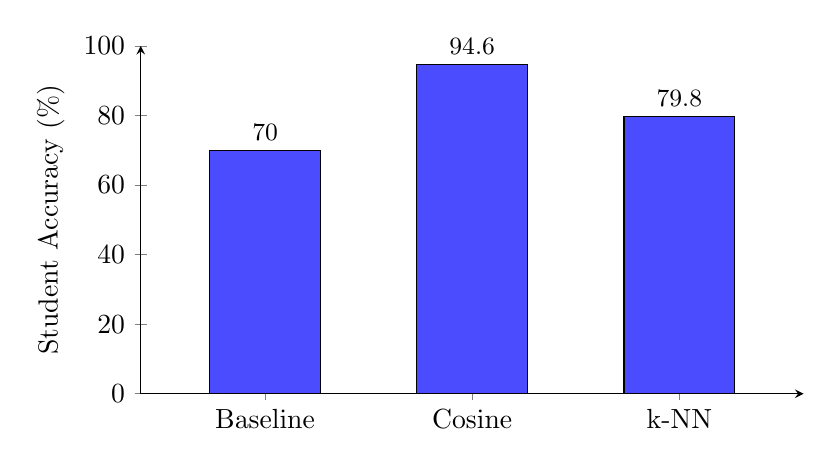
\begin{tikzpicture}
\begin{axis}[
    ybar,
    width=10cm,
    height=6cm,
    bar width=40pt,
    symbolic x coords={Baseline, Cosine, k-NN},
    xtick=data,
    ylabel={Student Accuracy (\%)},
    ymin=0, ymax=100,
    legend pos=north west,
    legend style={font=\small},
    nodes near coords,
    nodes near coords align={vertical},
    every node near coord/.append style={font=\small},
    axis x line=bottom,
    axis y line=left,
    enlarge x limits=0.3
]
\addplot[fill=blue!70] coordinates {
    (Baseline,70.0)
    (Cosine,94.6)
    (k-NN,79.8)
};
\end{axis}
\end{tikzpicture}
\end{center}

\begin{block}{Observation}
Cosine alignment: \textbf{+24.6\%} improvement (70.0\% $\to$ 94.6\%)
\end{block}

\end{frame}

%===============================================================================
\section{The Weight Initialization Problem}
%===============================================================================

\begin{frame}{Critical Experiment: Different Initialization}

\textbf{What happens if teacher and student start from different random seeds?}

\vspace{1em}

\begin{table}
\centering
\begin{tabular}{lcc}
\toprule
Configuration & Same Init & Different Init \\
\midrule
Baseline (no alignment) & 70.0\% & 6.7\% \\
Cosine ($\lambda=0.1$) & 94.6\% & 7.9\% \\
k-NN ($\lambda=0.1$) & 79.8\% & 7.8\% \\
\bottomrule
\end{tabular}
\end{table}

\vspace{1em}

\begin{block}{Observation}
\begin{itemize}
    \item Different initialization: all methods perform at baseline ($\sim$7\%, near-random)
    \item \textbf{-63\% drop} in performance
    \item Alignment methods provide \emph{no recovery}
\end{itemize}
\end{block}

\end{frame}

\begin{frame}{Can More Training Help?}

\textbf{Extended training with different initialization:}

\vspace{1em}

\begin{table}
\centering
\begin{tabular}{lcc}
\toprule
Method & 3 Epochs & 20 Epochs \\
\midrule
Baseline & 6.7\% & 6.2\% \\
Cosine Alignment & 7.9\% & 3.7\% \\
k-NN Alignment & 7.8\% & 7.8\% \\
\bottomrule
\end{tabular}
\end{table}

\vspace{1em}

\begin{itemize}
    \item \textbf{No recovery:} Performance stays near-random
    \item Cosine alignment actually degrades to 3.7\%
    \item More training time does not fix initialization mismatch
\end{itemize}

\end{frame}

%===============================================================================
\section{Weight Perturbation Analysis}
%===============================================================================

\begin{frame}{Weight Perturbation Sensitivity}

\textbf{How much weight divergence can the system tolerate?}

\vspace{0.5em}

Add Gaussian noise to student weights: $W_S \gets W_T + \mathcal{N}(0, \epsilon \cdot \text{scale}(W_T))$

\vspace{1em}

\begin{table}
\centering
\small
\begin{tabular}{lcc}
\toprule
Perturbation ($\epsilon$) & Student Accuracy & Zone \\
\midrule
0.0001 -- 0.02 & 96.5\% & \textcolor{green!60!black}{\textbf{Robust}} \\
0.03 -- 0.05 & 90.2\% & \textcolor{orange}{\textbf{Transition}} \\
$\geq$ 0.1 & 27.7\% & \textcolor{red}{\textbf{Failure}} \\
\bottomrule
\end{tabular}
\end{table}

\vspace{1em}

\begin{block}{Key Findings}
\begin{itemize}
    \item \textbf{Robust up to 2\%} weight-scale noise
    \item \textbf{Sharp transition} at 3-5\%
    \item \textbf{Performance collapse} beyond 10\%
\end{itemize}
\end{block}

\end{frame}

%===============================================================================
\section{Discussion}
%===============================================================================

\begin{frame}{Key Insights}

\begin{itemize}
    \item \textbf{Weight space compatibility is fundamental}
    \begin{itemize}
        \item Same initialization: essential for baseline subliminal learning
        \item Weight perturbation tolerance: $<$5\% scale
    \end{itemize}

    \vspace{0.5em}

    \item \textbf{Kernel alignment improves compatible systems}
    \begin{itemize}
        \item Cosine alignment: 70\% $\to$ 94.6\% (+24.6\%)
        \item k-NN alignment: 70\% $\to$ 79.8\% (+9.8\%)
        \item Cosine outperforms k-NN (global vs. local structure)
    \end{itemize}

    \vspace{0.5em}

    \item \textbf{Alignment cannot fix incompatible systems}
    \begin{itemize}
        \item Different initialization: all methods fail ($\sim$7\%)
        \item Extended training provides no recovery
        \item Operates at wrong level of abstraction
    \end{itemize}
\end{itemize}

\end{frame}

%===============================================================================
\section{Conclusion}
%===============================================================================

\begin{frame}{Summary}

\begin{itemize}
    \item AI reproduced subliminal learning from arXiv:2507.14805
    \begin{itemize}
        \item Baseline: 70\% accuracy on MNIST without labels
    \end{itemize}

    \vspace{0.5em}

    \item Does a kernel alignment method help with accuracy?
    \begin{itemize}
        \item Accuracy up to 94.6\%
    \end{itemize}

    \vspace{0.5em}

    \item Can kernel alignment compensate for different weight initializations?
    \begin{itemize}
        \item No -- both methods perform at baseline ($\sim$7\% accuracy)
        \item Weight space compatibility is fundamental
    \end{itemize}
\end{itemize}

\vspace{1em}

\begin{block}{I Learned}
Kernel alignment operates in representation space but cannot bridge incompatible weight spaces
\end{block}

\end{frame}

\begin{frame}{References \& Resources}

\textbf{Original Paper:}

\vspace{0.5em}

\small
\textit{``Subliminal Learning: Language models transmit behavioral traits via hidden signals in data''}\\
arXiv:2507.14805

\vspace{1.5em}

\normalsize
\textbf{This Implementation:}

\vspace{0.5em}

\begin{itemize}
    \item Code: github.com/Dezmon/SubliminalNetworks
    \item PyTorch implementation with MNIST
    \item Kernel alignment methods: Cosine (CKA-style) and k-NN
    \item Full experimental results in \texttt{analysis/} directory
\end{itemize}

\end{frame}

\begin{frame}[plain]
\centering
\Huge \textbf{Thank You}

\vspace{2em}

\Large Questions?

\vspace{2em}

\normalsize
\textbf{Code \& Results:} github.com/Dezmon/SubliminalNetworks

\textbf{Analysis:} See \texttt{analysis/EXPERIMENTAL\_RESULTS.md}
\end{frame}

%===============================================================================
% Backup Slides
%===============================================================================

\appendix

\begin{frame}[allowframebreaks]{Experimental Details}

\textbf{Architecture:}
\begin{itemize}
    \item Input: 784 (flattened 28×28 MNIST images)
    \item Hidden layers: 256 → 256 with ReLU activation
    \item Output: 10 regular logits + 3 auxiliary logits (default $m=3$)
    \item Initialization: He/Kaiming normal
\end{itemize}

\vspace{0.5em}

\textbf{Training:}
\begin{itemize}
    \item Optimizer: Adam (lr=0.001)
    \item Batch size: 64
    \item Teacher epochs: 3-5
    \item Student epochs: 3-20 (varied)
    \item Temperature: None (raw softmax)
\end{itemize}

\vspace{0.5em}

\textbf{Alignment:}
\begin{itemize}
    \item Layer: fc2 (second hidden layer, 256-dim)
    \item Weight: $\lambda = 0.1$ (default)
    \item Fresh random inputs for each alignment computation
\end{itemize}

\end{frame}

\begin{frame}{Complete Results Table}

\small
\begin{table}
\centering
\begin{tabular}{llcccc}
\toprule
Init & Method & Epochs & Teacher & Student & Gain \\
\midrule
Same & Baseline & 3 & 97.3\% & 70.0\% & +60.9\% \\
Same & Cosine-0.1 & 3 & 97.3\% & 94.6\% & +85.5\% \\
Same & k-NN-0.1 & 3 & 97.3\% & 79.8\% & +70.7\% \\
\midrule
Diff & Baseline & 3 & 97.5\% & 6.7\% & -2.4\% \\
Diff & Cosine-0.1 & 3 & 97.5\% & 7.9\% & -1.2\% \\
Diff & k-NN-0.1 & 3 & 97.5\% & 7.8\% & -1.4\% \\
\midrule
Diff & Baseline & 20 & 97.5\% & 6.2\% & -2.9\% \\
Diff & Cosine-0.1 & 20 & 97.5\% & 3.7\% & -5.4\% \\
Diff & k-NN-0.1 & 10 & 97.5\% & 7.8\% & -1.4\% \\
\bottomrule
\end{tabular}
\caption{Complete experimental results. ``Diff'' uses teacher seed=42, student seed=100.}
\end{table}

\end{frame}

\end{document}
